\chapter{Obtaining the weights}
\label{sect:data}
\section{Data used to obtain the weights}
\mbox{}\vspace{-\baselineskip}

The following sets of data were included into the EG.

\begin{enumerate}
\item Electroproduction data:
\begin{enumerate}
\item CLAS data at $E_{beam} = 2.445$ GeV,  $E_{beam} = 4$ GeV \cite{Ripani:2002ss}, \cite{Mokeev:2015lda};
\item CLAS data at $E_{beam} = 1.515$ GeV \cite{Fedotov:2008aa}, \cite{Mokeev:2008iw}, \cite{Mokeev:2012vsa}.
\end{enumerate}
\item Photoproduction data:
\begin{enumerate}
\item CLAS g11a data \cite{Golovach:note};
\item SAPHIR \& ABBHM data on integral cross sections \cite{Wu:2005wf}, \cite{ABBHHM:1968aa}.  
\end{enumerate}
\end{enumerate}

Single-differential electroproduction cross sections 1a~\cite{Ripani:2002ss} and 1b~\cite{Fedotov:2008aa} were fit with the JM model~\cite{Mokeev:2015lda},\cite{Mokeev:2008iw},\cite{Mokeev:2012vsa}, therefore all structure functions in Eq.~\eqref{eq:str_fun_decomp} obtained in this fit in a five-dimensional sense are used in TWOPEG.

Single-differential photoproduction cross sections 2a~\cite{Golovach:note} were also fit with the JM model that leads to the fact that at photon point $\sigma_{T}$ is also available from the fit in a five-dimensional sense. This is not the case for data-set 2b~\cite{Wu:2005wf}, for which only integral values of experimental cross section are available for different $W$ bins.

Figure~\ref{fig:gen_cover} shows which $W-Q^2$ areas are covered by these data-sets. The areas within red and lilac boundaries correspond to the electroproduction data 1a and 1b, respectively. The green and cyan lines along the horizontal $W$-axis correspond to the photoproduction data 2a and 2b, respectively. As it is seen in Fig.~\ref{fig:gen_cover} information about double pion production cross section exists only in very limited regions, while the major part of the $W-Q^2$ plane lacks information. In these areas, where information about double pion production cross section does not exist special interpolation and extrapolation procedures have been developed and applied in order to obtain reasonable cross section estimates (see Sect.~\ref{sect:cr_sect_extr_intr}). The brown line at $Q^2 = 1.3$ GeV$^2$ corresponds to the area for which the cross section was roughly estimated  from the JM model in a five-dimensional sense without relying on experimental data. It was done in order to extend the $W-Q^2$ coverage of TWOPEG further to the region of higher $W$-values, where no experimental data exists up to now.

\begin{figure}[htp]
\begin{center}
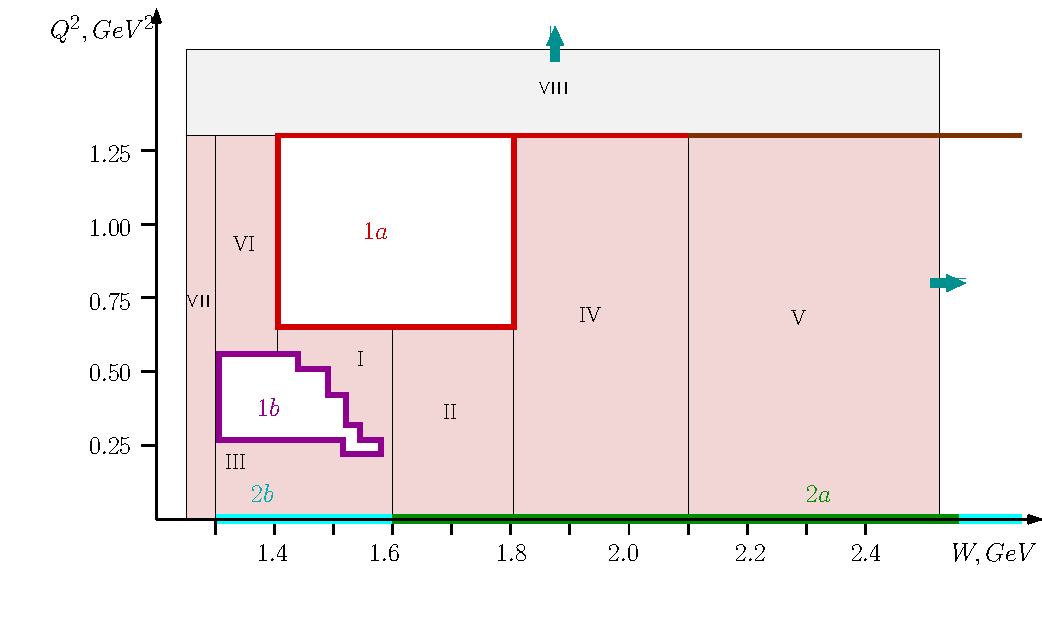
\includegraphics[width=16cm]{pictures/obt_weights/gen_cover.pdf}
\caption{\small $W-Q^2$ coverage of TWOPEG. The areas within red and lilac boundaries correspond to the electroproduction data 1a and 1b, respectively. The green and cyan lines along the horizontal $W$-axis correspond to the photoproduction data 2a and 2b, respectively. The brown line at $Q^2 = 1.3$ GeV$^2$ corresponds to the area for which the cross section was roughly estimated  from the JM model in a five-dimensional sense without relying on experimental data. The blue arrows indicate the extension to the higher $W$ and $Q^2$.} \label{fig:gen_cover}
\end{center}
\end{figure}


\section{Calculation of weights}
\label{sect:cr_sect_extr_intr}
%Regions covered by the data.
%Linear interpolations (four-dimensional and two-dimensional).

%Not covered regions.
%Fits of the $\sigma_{T}$ and $\varepsilon_{L}\sigma_{L}$. Function for $Q^{2}$ dependence from old EG. Usage of the integral cross sections in the photon point (SAPHIR). Cross sections at $W > 3$~GeV.

As it was mentioned in the previous section the single-fold differential cross sections from the data-sets 1a, 1b, and 2a were fit with the JM model, and as a result all structure functions from Eq.~\eqref{eq:str_fun_decomp} are available in a five-dimensional sense (from the photoproduction data-set 2a only $\sigma_{T}$ exists). Table~\ref{tab:mod_grid} shows the kinematical grid~\footnote[1]{Note that although the model cross section is differential in $(-cos \theta_{h})$, a grid that is equidistant in $\theta_{h}$ is used.}, in which the model structure functions were obtained.  


\begin{table}[h]%\scriptsize
\begin{center}
  \renewcommand{\arraystretch}{1.2}
\begin{tabular}{|c|c|c|c|c|c|c|c|}

\hline
Data & $Q^2$ values, & \# of $W$  & \# of $S_{12}$ & \# of $S_{23}$ & \# of $\theta_{h}$ & \# of $\alpha_{h}$  & \# of $\varphi_{h}$ \\
 set &  GeV$^2$ &  points &  points& points &  points &  points &  points\\
\hline
   &  0.65 & 17 &    &    &   &   & \\
1a &  0.95 & 17 & 12 & 12 & 6 & 6 & 1\\
   &  1.30 & 28 &    &    &   &   & \\
\hline
   &  0.225 & 4  &   &    &   &   &  \\
   &  0.275 & 11 &   &    &   &   &  \\
   &  0.325 & 10 &   &    &   &   &  \\
1b &  0.425 &  9 & 10&10  & 8 & 8 & 1\\
   &  0.475 &  8 &   &    &   &   &  \\
   &  0.525 &  8 &   &    &   &   &  \\
   &  0.575 &  6 &   &    &   &   &  \\
\hline
2a &  0.   &  30& 16&16  & 14&14 & 1\\
\hline
%2b &  ---   &    &---&--- &---&---&---\\
%\hline
\end{tabular}
\caption{\small Kinematical grid, in which the model structure functions are obtained. \label{tab:mod_grid}}
\end{center}
\end{table}

To  calculate the weight $f_{cr~sect}$ (see Eq.~\eqref{eq:weight_cr_sect}), means to estimate the value of the five-differential hadronic double pion cross section in the given corresponding 7-dimensional kinematical point ($W$,~$Q^2$,~$S_{12}$, $S_{23}$,~$\theta_{h}$,~$\varphi_{h}$,~$\alpha_{h}$). It in turn means that all structure functions from Eq.~\eqref{eq:str_fun_decomp} need to be estimated in that point.  The procedure of interpolation and extrapolation of the model structure functions into the desired point is described next. 


First, for each ($W$,~$Q^2$) point, where model structure functions are available, the four-dimensional linear interpolation is done between the points of the ($S_{12}$,~$S_{23}$,~$\theta_{h}$,~$\alpha_{h}$) grid. Then for the electroproduction data a two-dimensional linear interpolation is done between the points of the ($W$,~$Q^2$) grid, while for the photoproduction data a one-dimensional linear $W$-interpolation is done. As a result one can get the values of the structure functions for any arbitrary point located in the inner areas within the red and lilac boundaries and along the green line in Fig.~\ref{fig:gen_cover}. 

Region I. The two-dimensional linear ($W$,~$Q^2$) interpolation is also performed between the regions 1a and 1b for $1.4 < W < 1.6$ GeV. 

In order to estimate the values of the structure functions in other regions (colored by pink in Fig.~\ref{fig:gen_cover} and numbered by roman numerals) the special procedures should be applied.

Region II. Let's consider the region $1.6 < W < 1.825$ GeV and $0 < Q^2 < 0.65$ GeV$^2$. For $Q^2 = 0.65$~GeV$^2$ the full set of five-dimensional structure functions are available from the model analysis of data-set 1a. For the photon point only $\sigma_{T}$ is available from the model analysis of data-set 2a. In order to estimate the value of all structure functions in any point of this region a procedure, which contains the following steps was developed.

\begin{itemize}

\item The integral values of model structure function $\sigma_T$ in three $Q^2$ points (0, 0.65, and 0.95~GeV$^2$) were fit with the following function for each $W$ point individually:
\begin{equation}
F_{T}(Q^2) = a_{0}\left (Q^2+a_1 \right )^{a_2}+a_{3},
\label{eq:q2_dep_fit_sig_t}
\end{equation}

where $a_{0}$, $a_{1}$, $a_{2}$, and $a_{3}$ are free fit parameters.

The result of this fit for $W = 1.7125$ GeV is shown in Fig.~\ref{fig:sig_t_l_fit} (left side). The black points are the integrated values of model structure function $\sigma_{T}$ and the red curve is the fit function $F_{T}(Q^2)$. 


Then the five-differential structure function $\sigma_{T}$ can be scaled between the $Q^2$ boundaries to any arbitrary $Q^2$ point along the obtained $Q^2$ dependence. But since $\sigma_{T}$ exists in a five-dimensional sense at both boundaries ($Q^2 = 0.65$~GeV$^2$ and $Q^2 = 0$~GeV$^2$), it can be scaled from both sides. To avoid loss of information about the evolution of the differential cross section shape with $Q^2$, it was decided to mix these two scaled structure functions at each $Q^2$ point. Thus the differential structure function in arbitrary point $0 < Q^2 < 0.65$~GeV$^2$ is given by

\begin{equation}
\frac{d^5\sigma_{T}}{d^5\tau}\left ( Q^2 \right ) = \frac{Q^2}{0.65}\frac{d^5\sigma_{T}}{d^5\tau}\left ( 0.65 \right )\frac{F_{T}(Q^2)}{F_{T}(0.65)}+\frac{0.65-Q^2}{0.65}\frac{d^5\sigma_{T}}{d^5\tau}\left ( 0 \right )\frac{F_{T}(Q^2)}{F_{T}(0)}.
\label{eq:q2_dep_fit_sig_t}
\end{equation}

The first term corresponds to the value of $\sigma_{T}$, which is scaled from the $Q^2=0.65$~GeV$^2$ edge, while the second one is scaled from the $Q^2 = 0$~GeV$^2$ edge. The first fraction in each term corresponds to the mixing coefficient, which forces the term to completely dominate at its own edge and to vanish at the opposite edge. The last fraction in each term corresponds to the integral scaling. All numerical values in Eq.~\eqref{eq:q2_dep_fit_sig_t} are given in GeV$^2$.

\begin{figure}[htp]
\begin{center}
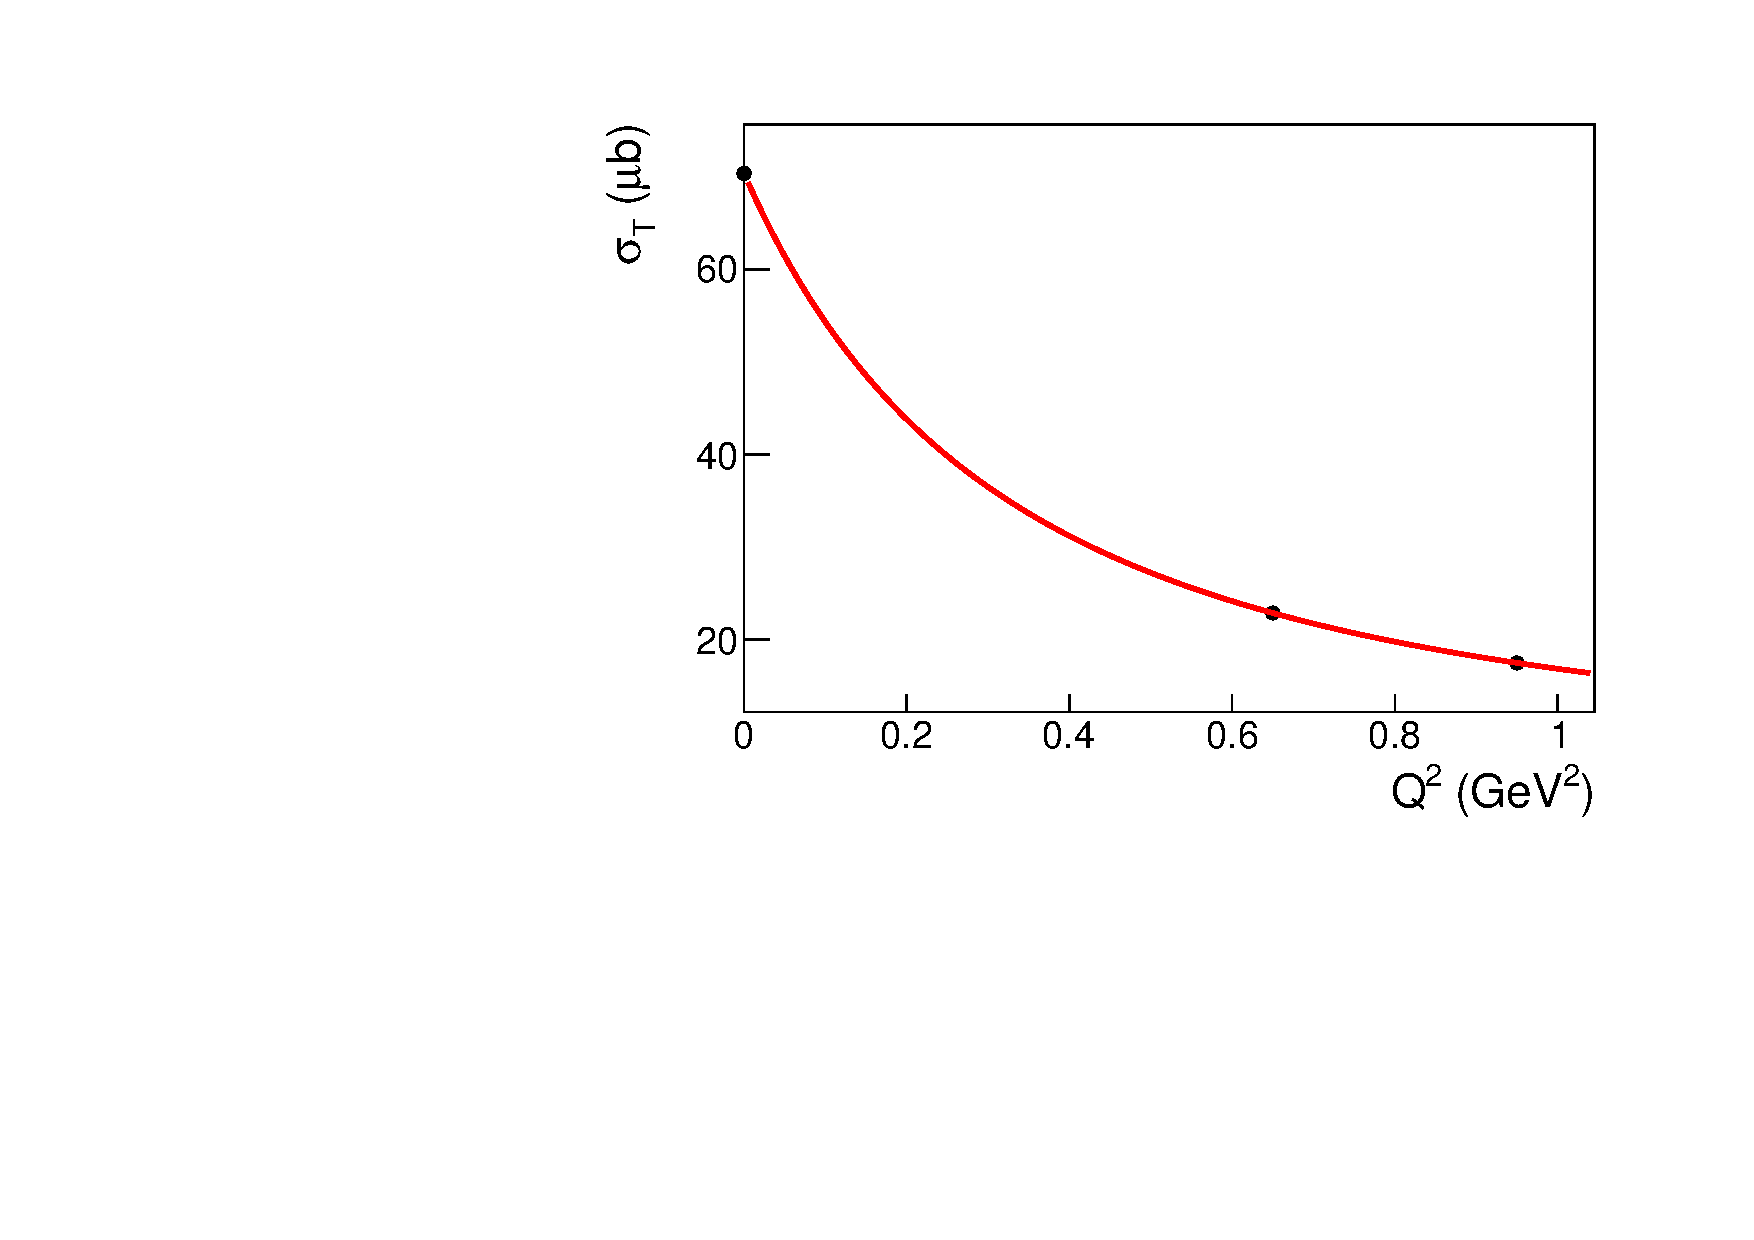
\includegraphics[height=0.32\textwidth]{pictures/obt_weights/sigma_t_fit_17125.pdf}
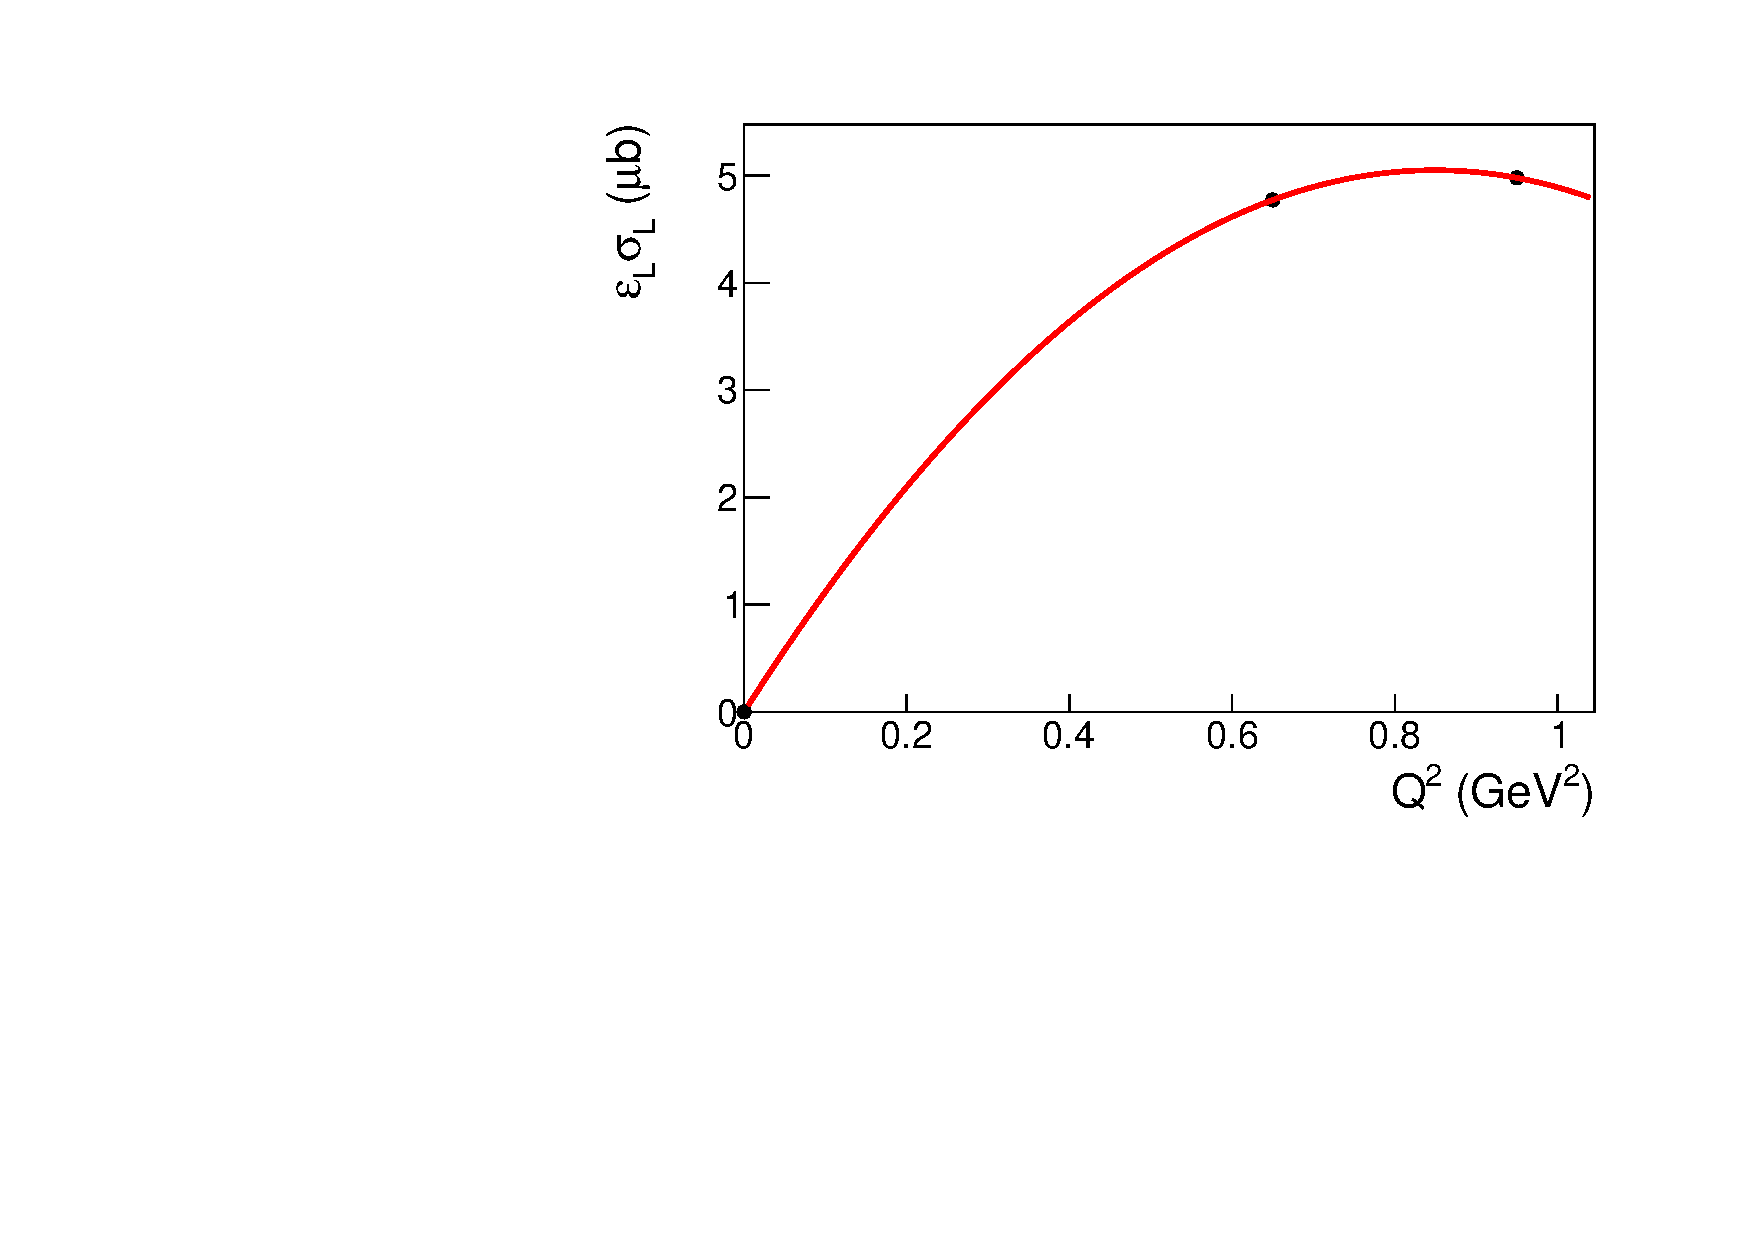
\includegraphics[height=0.32\textwidth]{pictures/obt_weights/sigma_l_fit_17125.pdf}
\caption{\small Left side: fit of the integrated values of model structure function $\sigma_{T}$ (black points) with the function given by Eq.~\eqref{eq:q2_dep_fit_sig_t} for the $W = 1.7125$ GeV. The red curve corresponds to the function $F_{T}(Q^2)$, which is the fit result. Right side: fit of $\varepsilon_{L}\sigma_L$ with a second order polynom for $W = 1.7125$ GeV. The values of $\varepsilon_{L}$ are calculated for a beam energy of 2.445~GeV, with which the experiment 1a ran. The red curve corresponds to the function $F_{L}(Q^2)$, which is the fit result. } \label{fig:sig_t_l_fit}
\end{center}
\end{figure}

\item For the structure function $\sigma_{L}$ the situation is more complicated, since no information about it exists at the photon point and for this reason one can neither perform the fit nor the cross section mixing as described in the previous step. Hence the procedure should be modified. The modification is made based on the fact that although the information about the $\sigma_{L}$ behavior close to the photon point is unknown, the combination $\varepsilon_{L}\sigma_{L}$ must definitely vanish at $Q^2 = 0$~GeV$^2$. Therefore, the values of the combination $\varepsilon_{L}\sigma_L$ in the three $Q^2$ points (0, 0.65, and 0.95~GeV$^2$) were fit with a second order polynom. The result of this fit for $W = 1.7125$ GeV is shown in Fig.~\ref{fig:sig_t_l_fit} (right side). The black points are the values of $\varepsilon_{L}\sigma_L$, where $\sigma_{L}$ is the integrated model structure function and $\varepsilon_{L}$ is defined in the context of Eq.~\eqref{eq:str_fun_decomp}. The red curve is the resulting fit function $F_{L}(Q^2)$.

Figure~\ref{fig:sig_gen} shows the event distributions of TWOPEG, which are obtained based on this approach. Left plot shows the $Q^2$ dependence of the integral  quantities $\sigma_{T}$ (blue curve), $\varepsilon_{L}\sigma_{L}$ (green curve) and $\sigma_{T}+\varepsilon_{L}\sigma_{L}$ (red curve) in comparison with the model points. As it is seen in this plot the longitudinal term $\varepsilon_{L}\sigma_{L}$ gives rather small contribution to the full cross section. Right plot shows the estimated behavior of the structure function $\sigma_{L}$. 

\begin{figure}[htp]
\begin{center}
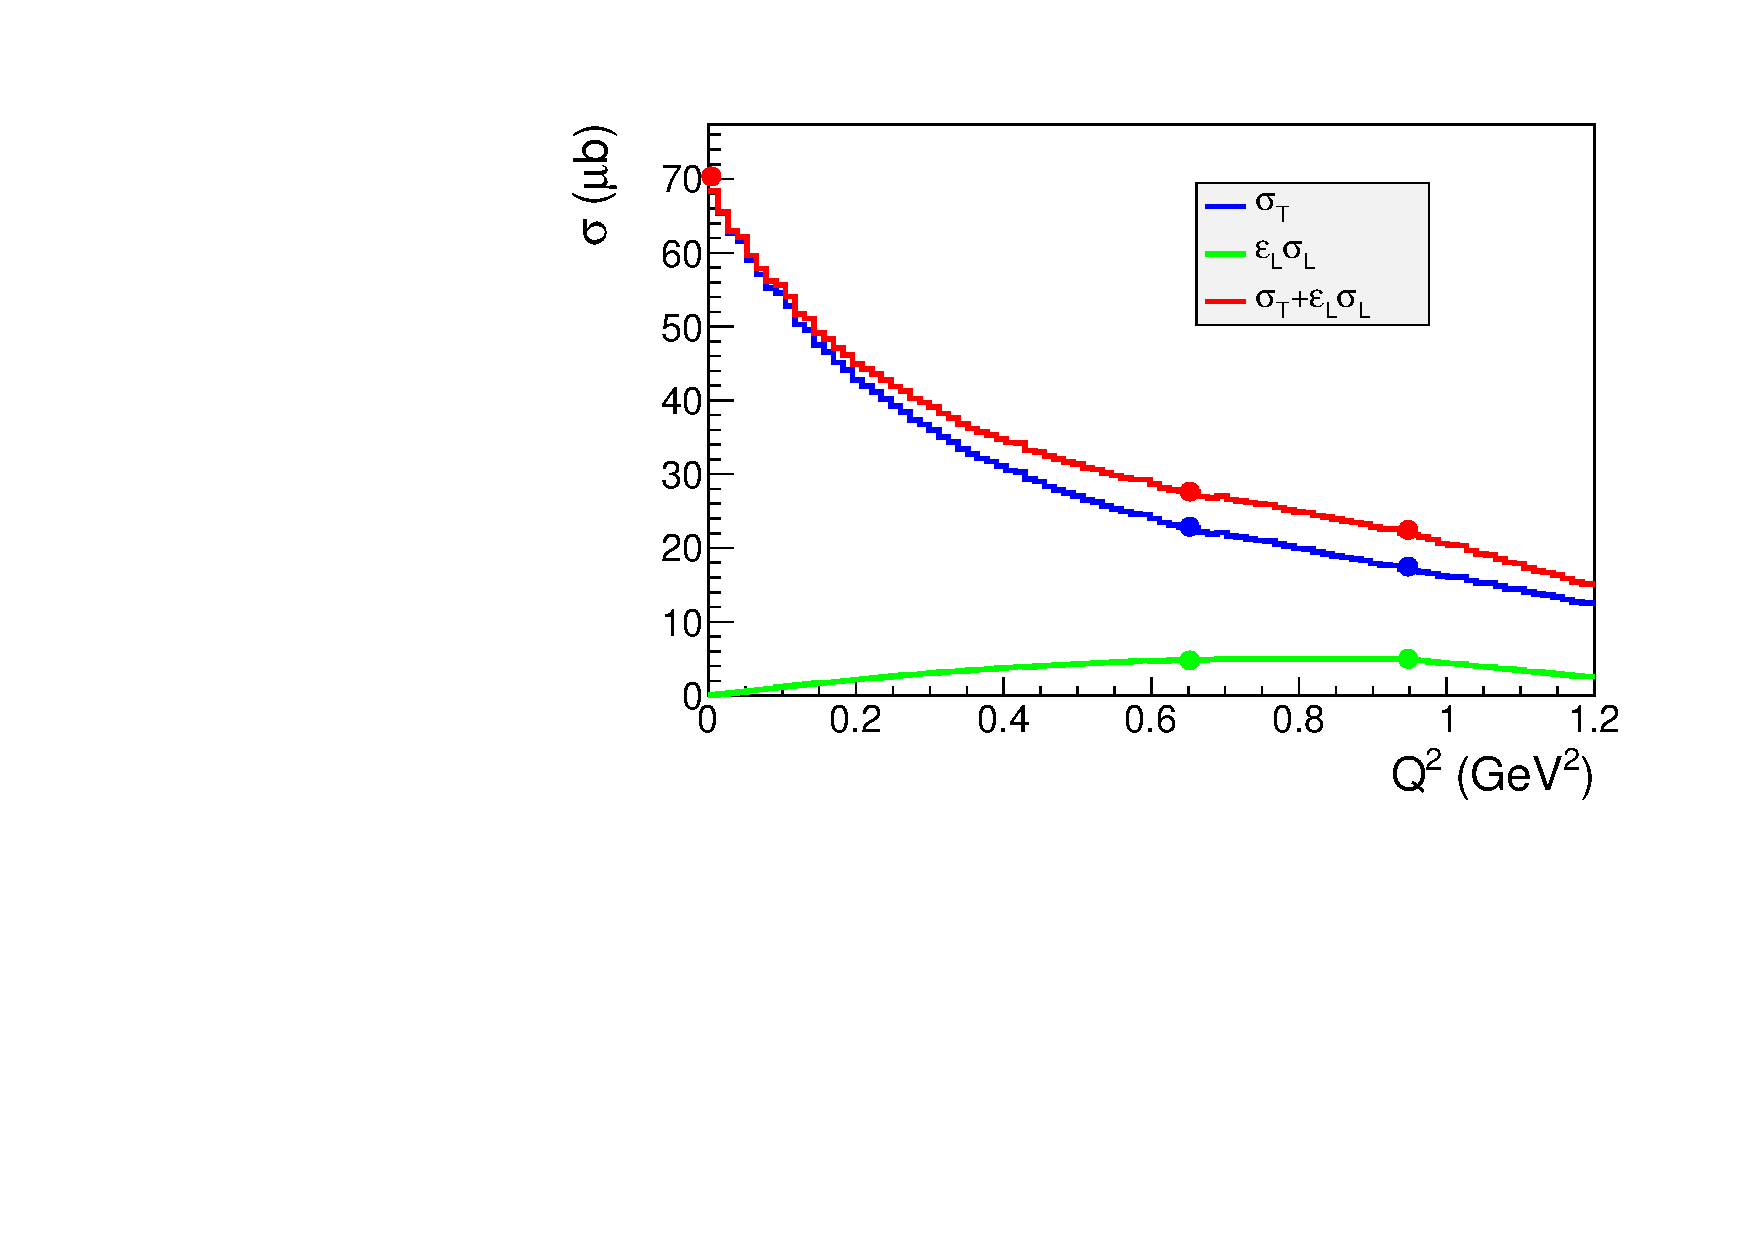
\includegraphics[height=0.35\textwidth]{pictures/obt_weights/t_epsl_tot_gen_mod_comp.pdf}
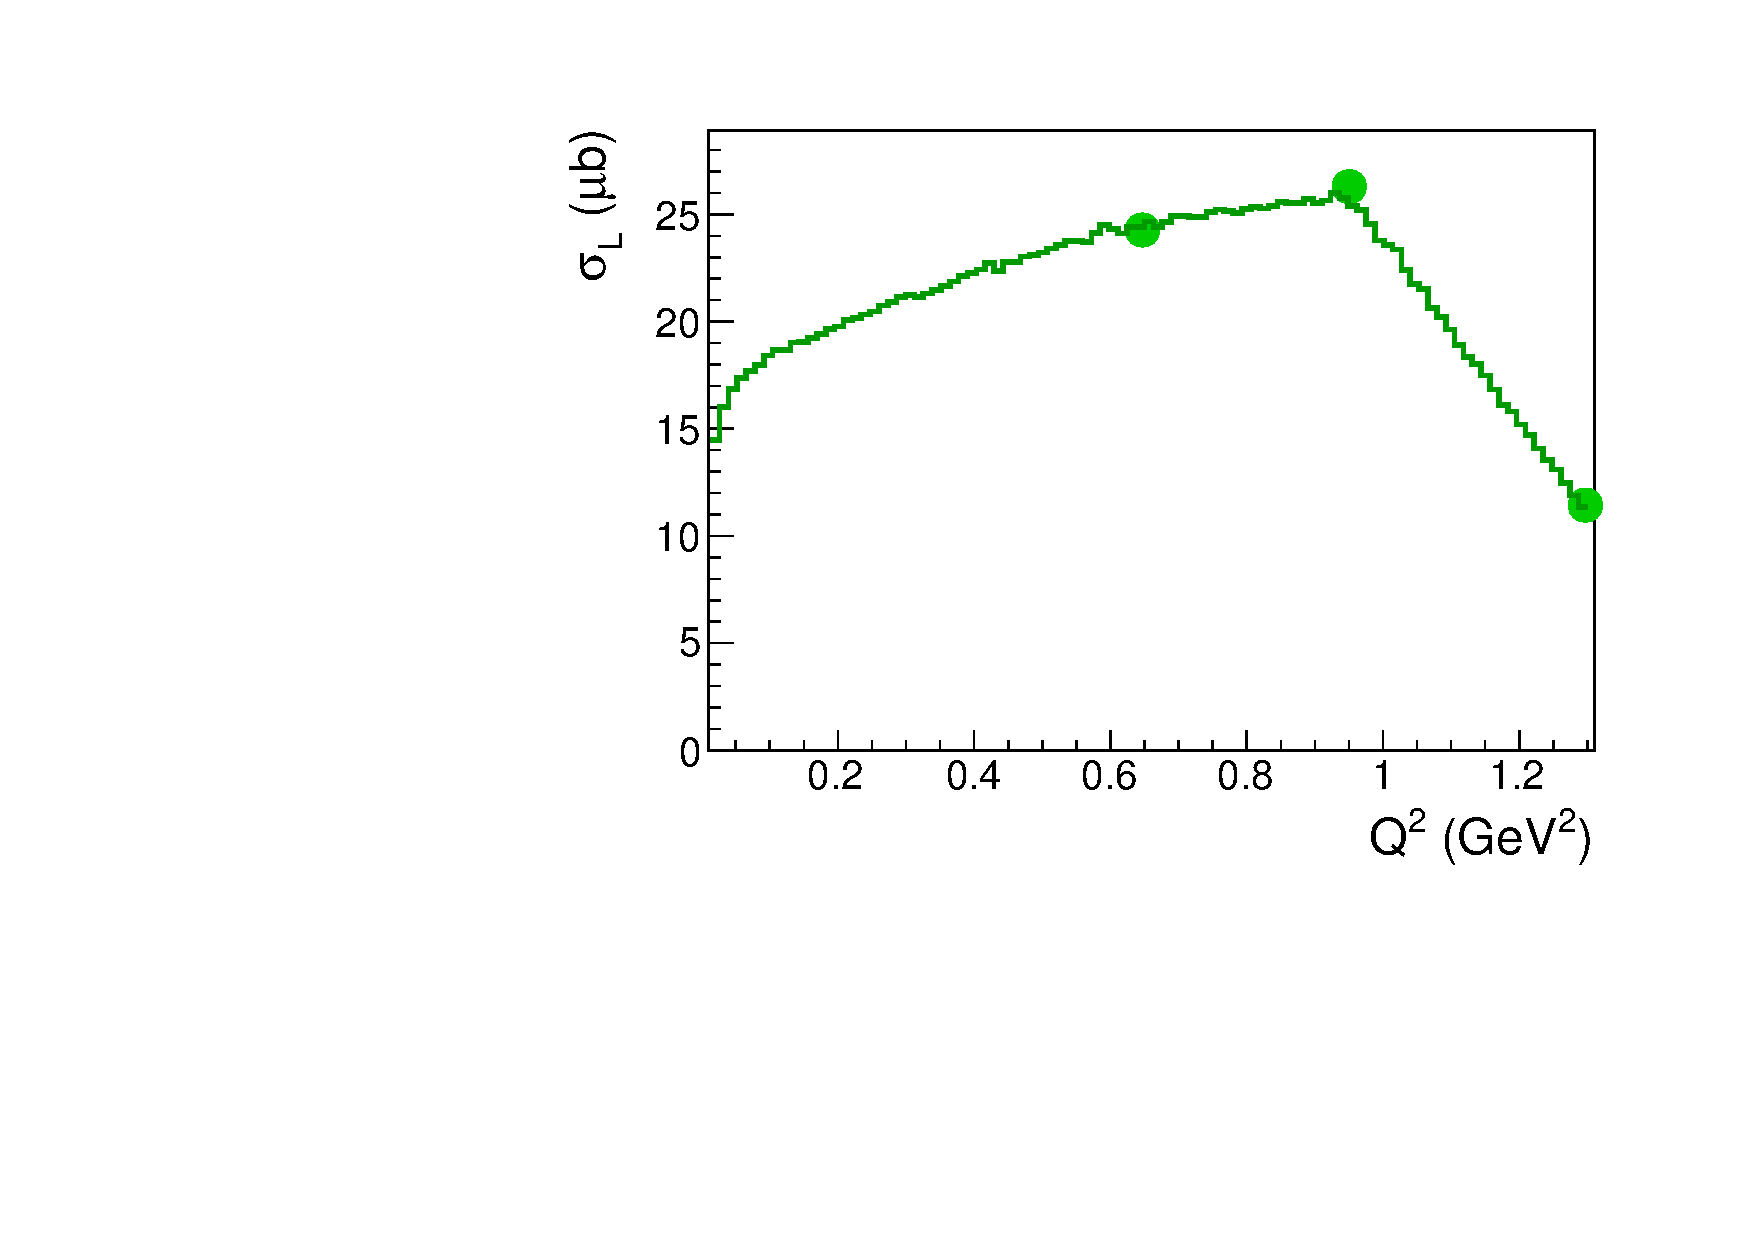
\includegraphics[height=0.35\textwidth]{pictures/obt_weights/sig_l_no_epsl.pdf}
\caption{\small $Q^2$ dependence of different contributors to the full integral cross sections. Comparison between the event distributions of TWOPEG (curves) with the JM model values (points). Left side: integral $\sigma_{T}$ (blue), $\varepsilon_{L}\sigma_{L}$ (green), and $\sigma_{T}+\varepsilon_{L}\sigma_{L}$ (red) as a function of $Q^2$. The values of $\varepsilon_{L}$ are calculated for a beam energy of 2.445~GeV, with which the experiment 1a ran. Right side: the structure function $\sigma_{L}$ as a function of $Q^2$. For both plots curves are obtained with TWOPEG for the $W$-bin [1.7, 1.725]~GeV, while the points are for the JM model at $W=1.7125$~GeV.  } \label{fig:sig_gen}
\end{center}
\end{figure}

Since $\sigma_{L}$ exists in a five-dimensional sense at $Q^2 = 0.65$~GeV$^2$ the differential structure function $\sigma_{L}$ in any point at $0 < Q^2<0.65$~GeV$^2$ can be obtained by

\begin{equation}
\frac{d^5\sigma_{L}}{d^5\tau}\left ( Q^2 \right ) = \frac{d^5\sigma_{L}}{d^5\tau}\left ( 0.65\;{\rm GeV^2} \right )\frac{F_{L}(Q^2)}{F_{L}(0.65\;{\rm GeV^2})}\frac{\varepsilon_{L}(2.445\;{\rm GeV},0.65\;{\rm GeV^2})}{\varepsilon_{L}(2.445\;{\rm GeV},Q^2)},
\label{eq:q2_dep_fit_sig_l}
\end{equation}

where the value of $\varepsilon_{L}$ is calculated here for $E_{beam} = 2.445$~GeV in order to satisfy the conditions, under which the experiment 1a was made.



\item The terms in Eq.~\eqref{eq:str_fun_decomp} that correspond to other structure functions are also forced by the coefficients in front of them to vanish at $Q^2 = 0$~GeV$^2$. Hence these structure functions exist in five-dimensional sense only at the $Q^2 = 0.65$~GeV$^2$ edge. Their contribution into the full cross section is an order of a magnitude lower than the contribution from the first (transverse) and second (longitudinal) terms, thus there is no need to develop complex procedure for the purpose of their extrapolation to the region $Q^2 < 0.65$~GeV$^2$. For this purpose the following approximate $Q^2$ dependence is used:

 \begin{equation}
F_{approx}(Q^2) = \frac{1}{\left (1+\frac{Q^2}{0.7~GeV^2}\right )^{2}},
\label{eq:q2_dep}
\end{equation}

The differential structure functions in any point at $0 < Q^2<0.65$~GeV$^2$ can be obtained in this way:

 \begin{equation}
\frac{d^5\sigma_{X}}{d^5\tau}\left ( Q^2 \right ) = \frac{d^5\sigma_{X}}{d^5\tau}\left ( 0.65\;{\rm GeV^2} \right )\frac{F_{approx}(Q^2)}{F_{approx}(0.65\;{\rm GeV^2})},
\label{eq:sig_x_acale}
\end{equation}

where $\sigma_X$ corresponds to $\sigma_{TT}$, $\widetilde{\sigma}_{TT}$, $\sigma_{TL}$, and $\widetilde{\sigma}_{TL}$.

\item Last step of the procedure is to perform linear one-dimensional interpolation of all structure functions into the given $W$ point.

\end{itemize}


After that in any arbitrary point in the region of $1.6 < W < 1.825$ GeV and $0<Q^2<0.65$ GeV$^2$ all structure functions are estimated in a multi-dimensional sense.


Region III. In the region of $1.3 < W < 1.6$ GeV and $0 < Q^2 < 0.275$ GeV$^2$ the same procedure as for region II is applied, with the exception of $\sigma_{T}$ mixing, which can not be done, since structure function $\sigma_{T}$ is available in a five-dimensional sense only at $Q^2 = 0.275$~GeV$^2$, and at $Q^2 = 0$~GeV$^2$ just integral values of $\sigma_{T}$ are known from the data-set 2b (cyan line in Fig.~\ref{fig:gen_cover}). This leads to the fact that the shapes of all differential structure functions for $Q^2 < 0.275$~GeV$^2$ remain the same as at  $Q^2 = 0.275$~GeV$^2$, although their absolute normalization changes properly due to the integral scaling.

Region IV. Now let's proceed to the region of $1.825 < W < 2.1$ GeV and $0<Q^2<1.3$ GeV$^2$. For $Q^2 = 1.3$~GeV$^2$ the full set of five-dimensional structure functions are available from the model analysis of data-set 1a. For the photon point only $\sigma_{T}$ is available from the model analysis of the data-set 2a. Therefore, a procedure similar to that described above for the region II can be applied here. The only difference is that the $Q^2$ dependence of all structure functions was not obtained by the fit of the corresponding integral values, but was taken to be the same as the one at $W = 1.8125$~GeV. This was done for the following reasons. A fit of the integral $\sigma_{T}$ structure function is not expected to be reliable, since for $\sigma_{T}$ model prediction exists only for two $Q^2$ points (at $Q^2 = 1.3$~GeV$^2$ and $Q^2 = 0$~GeV$^2$), which are very far from each other. For the longitudinal part of the cross section no fit can be done, since the model prediction exits only at a single point, $Q^2 = 1.3$~GeV$^2$. 

Region V. The same procedure (IV) is also used for the region of $W > 2.1$ GeV and $0<Q^2<1.3$ GeV$^2$ with the only distinction that for $W > 2.1$~GeV and $Q^2 = 1.3$~GeV$^2$ the five-dimensional structure functions were roughly estimated by the JM model without relying on experimental data, since no data exists there (the brown line in Fig.~\ref{fig:gen_cover}). The same was done also for $W > 2.5$~GeV and $Q^2 = 0$~GeV$^2$, but here the information about integral photoproduction cross sections (data-set 2b shown with the cyan line in Fig.~\ref{fig:gen_cover}) was used. Thereby TWOPEG works up to $W = 4.5$~GeV, but the higher the value of $W$ is, the less reliable the cross section shape becomes.

Region VI. For the region of $1.3 < W < 1.4$~GeV and $0.575 < Q^2 < 1.3$~GeV$^2$ the five-differential structure functions, which exist at $Q^2 = 0.575$~GeV$^2$ from the model analysis of data-set 1b, were scaled to the region $Q^2 > 0.575$~GeV$^2$ with the $Q^2$ dependence that is taken to be the same as at $W = 1.4125$~GeV. This dependence is linear between the $Q^2$ points 0.575, 0.65, 0.95, and 1.3~GeV$^2$. Thus the shape of all differential structure functions remains the same in this region, and only integral scaling takes place.

Region VII. In order to extend the EG coverage closer to the threshold the following was done in the region of $1.2375 < W < 1.3125$~GeV and $0.005 < Q^2 < 1.3$~GeV$^2$. Three extra $W$ points at 1.2375, 1.2625, and 1.2875 GeV were added. The structure functions at these points are taken to be the same as at the point $W = 1.3125$~GeV, except for two modifications: 1) invariant mass distributions are forced to shrink as $W$ decreases and 2) integral scaling is applied in order to force the integral cross section vanish at the threshold. The $Q^2$ dependence remains the same as at $W=1.3125$~GeV. A linear $W$ interpolation is done between the additional $W$ points.  
 


Region VIII. In regard to the extension of the EG coverage to the region with $Q^2 > 1.3$~GeV$^2$ the simple approximate $Q^2$ dependence given by Eq.~\eqref{eq:q2_dep} is used. The structure functions in this case are given by


\begin{equation}
\frac{d^5\sigma_{X}}{d^5\tau}\left ( Q^2  > 1.3~{\rm GeV^2} \right ) = \frac{d^5\sigma_{X}}{d^5\tau}\left ( 1.3\;{\rm GeV^2} \right )\frac{F_{approx}(Q^2)}{F_{approx}(1.3\;{\rm GeV^2})},
\label{eq:sig_x_acale_gt_1_3}
\end{equation}

where $\sigma_X$ corresponds to $\sigma_{T}$, $\sigma_{L}$, $\sigma_{TT}$, $\widetilde{\sigma}_{TT}$, $\sigma_{TL}$ and $\widetilde{\sigma}_{TL}$.

The shape of all differential structure functions for $Q^2 > 1.3$~GeV$^2$ remains the same as at  $Q^2 = 1.3$~GeV$^2$, but their absolute values decrease according to the integral scaling given by Eq.~\eqref{eq:sig_x_acale_gt_1_3}.

After all these steps adapted to the different $W-Q^2$ regions shown in Fig.~\ref{fig:gen_cover} are applied, all structure functions can be obtained at any arbitrary point for $W$ in [1.2375, 4.5375]~GeV and $Q^2 > 0.005$~GeV$^2$. The resulting structure functions can be combined into the full five-differential hadronic cross section according to Eq.~\eqref{eq:str_fun_decomp} for any particular beam energy given as an input parameter. To obtain the weight factor for each generated event, this cross section must be multiplied by the virtual photon flux given by Eq.~\eqref{flux} in order to obtain the proper electron scattering cross section, which leads to

\begin{equation}
f_{cr~sect} = 2\pi^3(S_{12}^{max}-S_{12}^{min})(S_{23}^{max}-S_{23}^{min})\Gamma_{v}(W,Q^2)\frac{d^{5}\sigma_{v} }{d^{5}\tau},
\label{eq:weight_cr_sect}
\end{equation}
%~\footnote[1]{It needs to be mentioned that if one wants to generate }
where $\frac{d^{5}\sigma_{v} }{d^{5}\tau}$ is the full hadronic cross section given by Eq.~\eqref{eq:str_fun_decomp} and $\Gamma_{v}(W,Q^2)$ the virtual photon flux given by Eq.~\eqref{flux}. Other factors are introduced in order to make the generated events consistent with the experimental ones and to force them to give the integral cross section value upon a weighted summation of events in $W$, $Q^2$ bin. 
%If the weight is normalized in a way given by Eq.~\eqref{eq:weight_cr_sect} the generated events can be treated exactly in the same way as the experimental ones. 
The $W$ dependent factors $(S_{12}^{max}-S_{12}^{min})$ and $(S_{23}^{max}-S_{23}^{min})$ are especially essential for the correct weight propagation. $S_{12}^{min},~S_{12}^{max},~S_{23}^{min},~S_{23}^{max}$ are the minimal and maximal values of the corresponded invariant mass squared at the given $W$ point.   With these factors  one can get the proper $W$ dependence of the integrated cross section automatically by the weighted sum of events in the particular $W$ bins.

It also needs to be mentioned that the multiplication by the virtual photon flux $\Gamma_{v}$ in Eq.~\eqref{eq:weight_cr_sect} corresponds to the mode, where the input flag $F_{flux} = 1$. In this case TWOPEG simulates events that are collected during the electron scattering experiments. This mode must be used if the EG is used for the modeling of experiment, for example efficiency evaluation.

But TWOPEG can also work in the mode $F_{flux} = 0$, in which the weight $f_{cr~sect}$ is not multiplied by the virtual photon flux $\Gamma_{v}$ in Eq.~\eqref{eq:weight_cr_sect}. In that case the weight corresponds to the hadronic cross section under the influence of virtual photons. This mode is convenient   if one wants to unfold the hadronic cross section value from the EG distributions (see Sect.~\ref{unfold} for details).  



